\documentclass[../presentation.tex]{subfiles} % Parent file
\graphicspath{{\subfix{../images/}}} % Images path

\begin{document}

\section{Segmentation Models} % This if you want to set the gray section title


% Slide 1 ──────────────────────────────────────────────────────────────────────
\begin{frame}[t] % t: top alignment of the slide content

	\frametitle{U-Net Models}

	$3$ models for the segmentation task:

	% \only<1->{
	% \begin{cbox}
	% 	\begin{itemize}
	% 		\item \bft{Classic U-Net}: \itt{\gray{baseline U-Net model architecture}}
	% 	\end{itemize}
	% \end{cbox}
	% }

	% \only<2->{
	% \begin{cbox}
	% 	\begin{itemize}
	% 		\item \bft{Improved U-Net}: \itt{\gray{small improvements, less
	% 			parameters}}
	% 	\end{itemize}
	% \end{cbox}
	% }

	% \only<3->{
	% \begin{cbox}
	% 	\begin{itemize}
	% 		\item \bft{Attention U-Net}: \itt{\gray{attention mechanism added}}
	% 	\end{itemize}
	% \end{cbox}
	% }

	\begin{itemize}
		\setlength{\itemsep}{0.8ex}
		\only<1->{\item \bft{Classic U-Net}: \itt{\gray{baseline U-Net model
		architecture}}}
		\only<2->{\item \bft{Improved U-Net}: \itt{\gray{small improvements, less
		parameters}}}
		\only<3->{\item \bft{Attention U-Net}: \itt{\gray{attention mechanism
		added}}}
\end{itemize}

	\vspace{-2ex}

	\only<4->{
		\begin{figure}
			\centering
			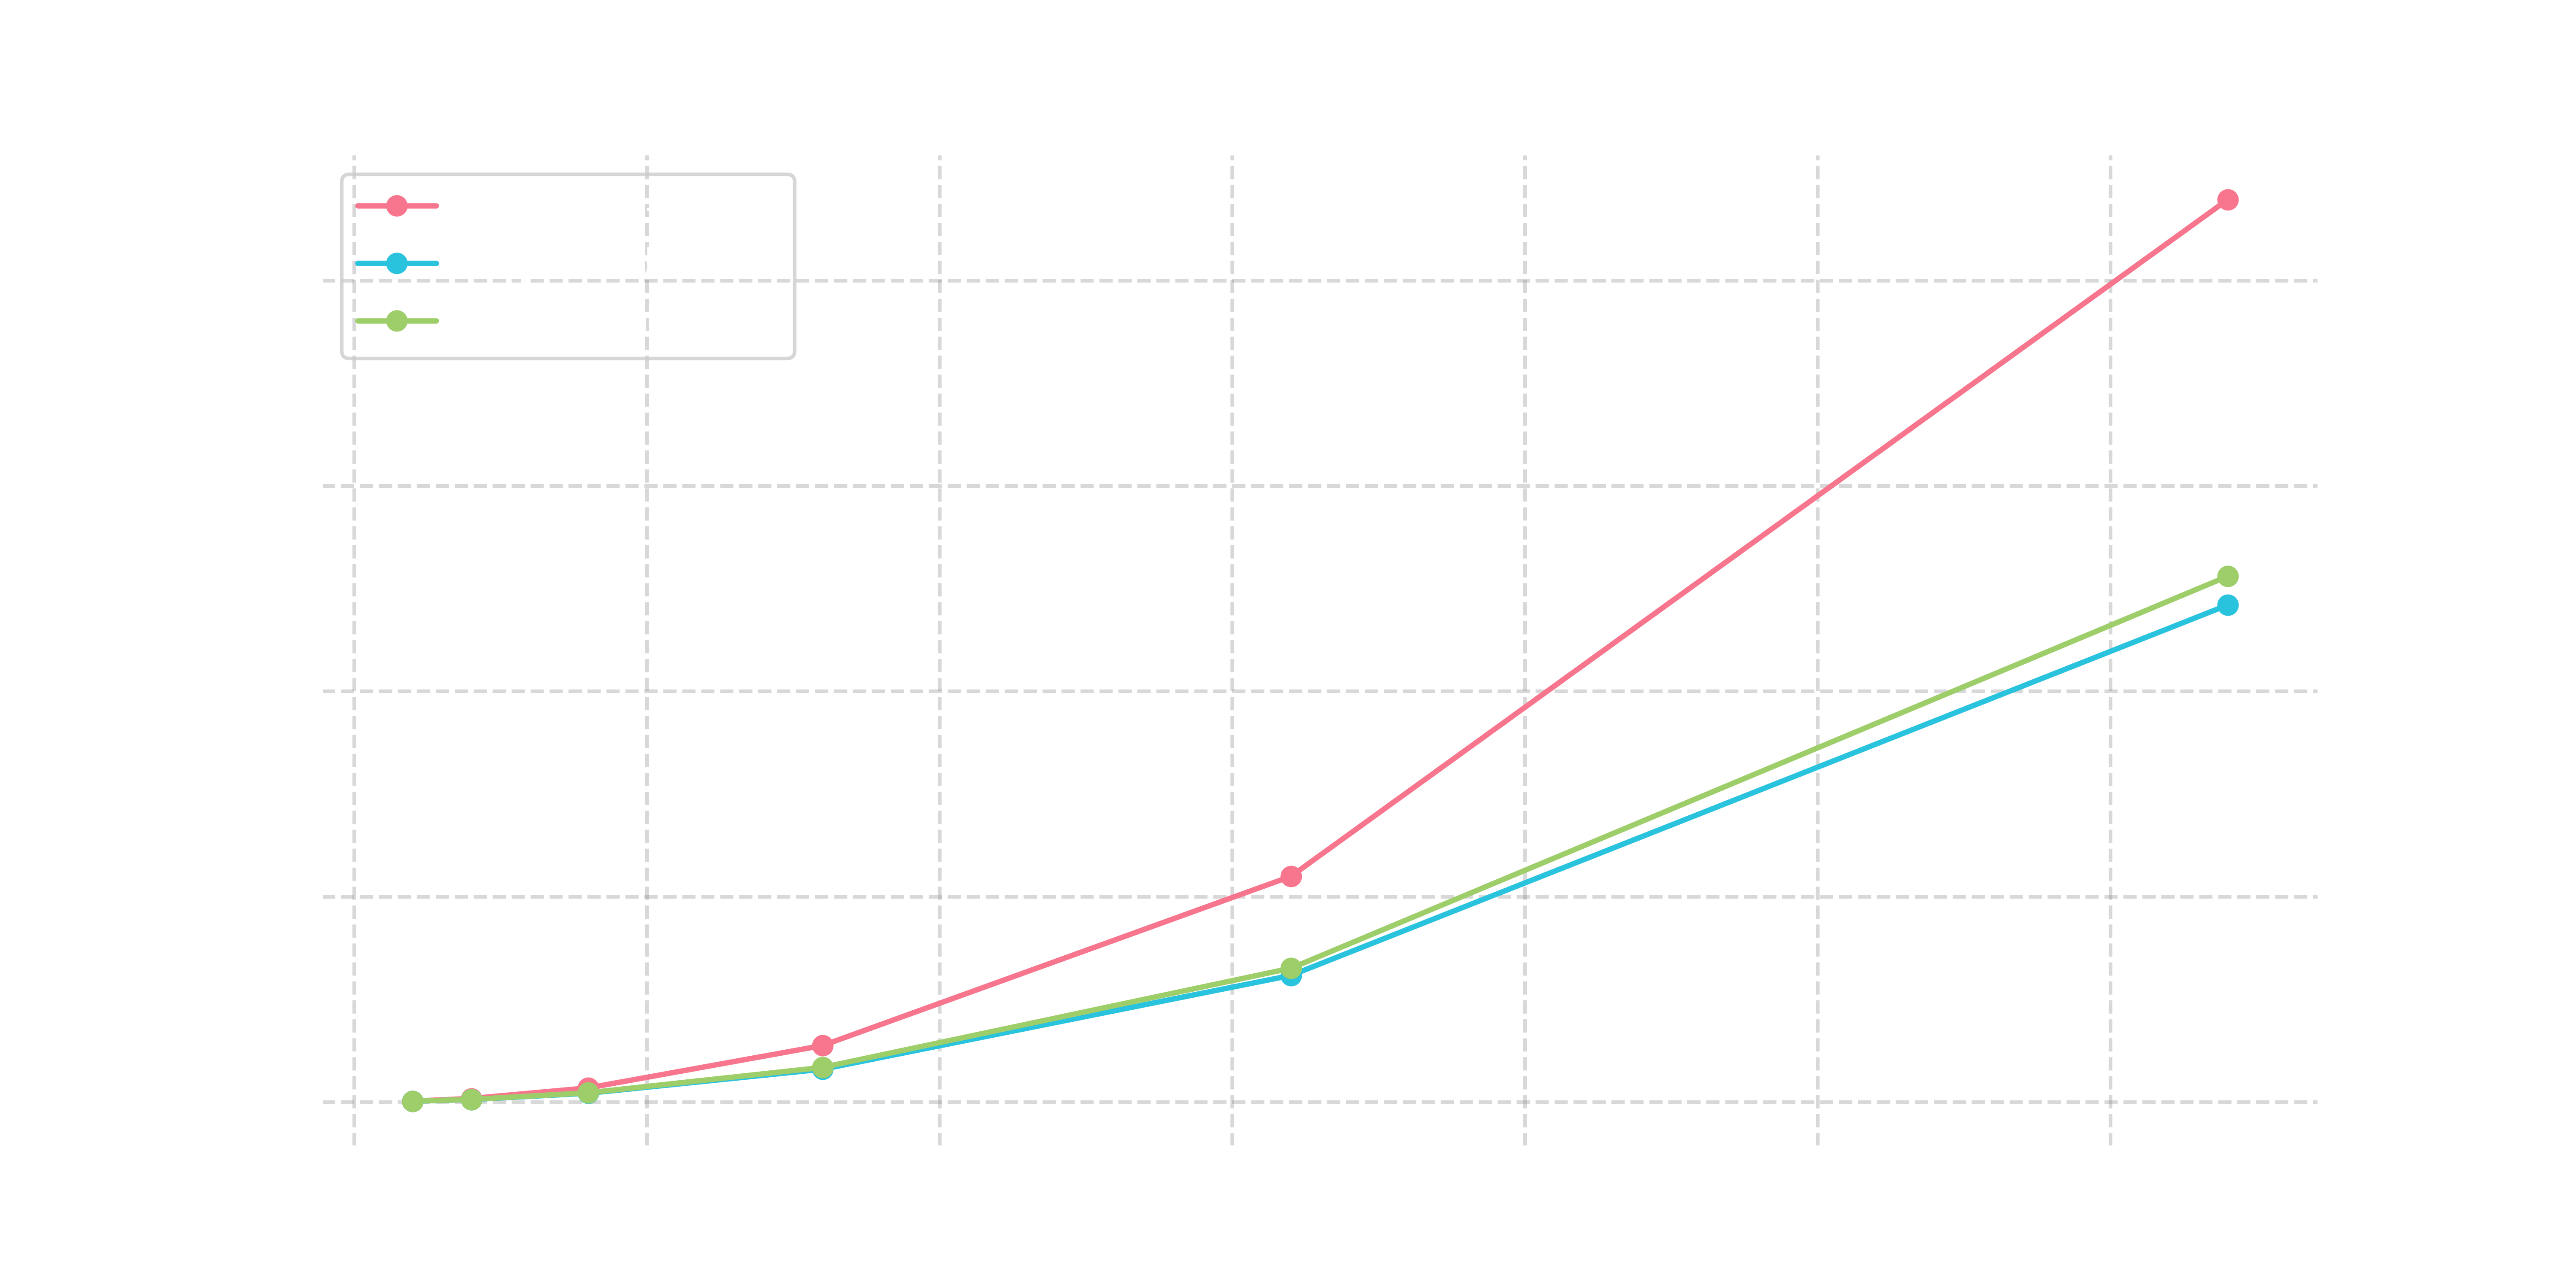
\includegraphics[width=\textwidth]{parameters_vs_filters.png}
		\end{figure}
	}

\end{frame}


% Slide 2 ──────────────────────────────────────────────────────────────────────
\begin{frame}

	\frametitle{Classic U-Net}

	% TODO: Replace this figure with TikZ picture and correct numbers
	% + in the tikz picture write the important elements highlighted in the speech
	\begin{figure}
		\centering
		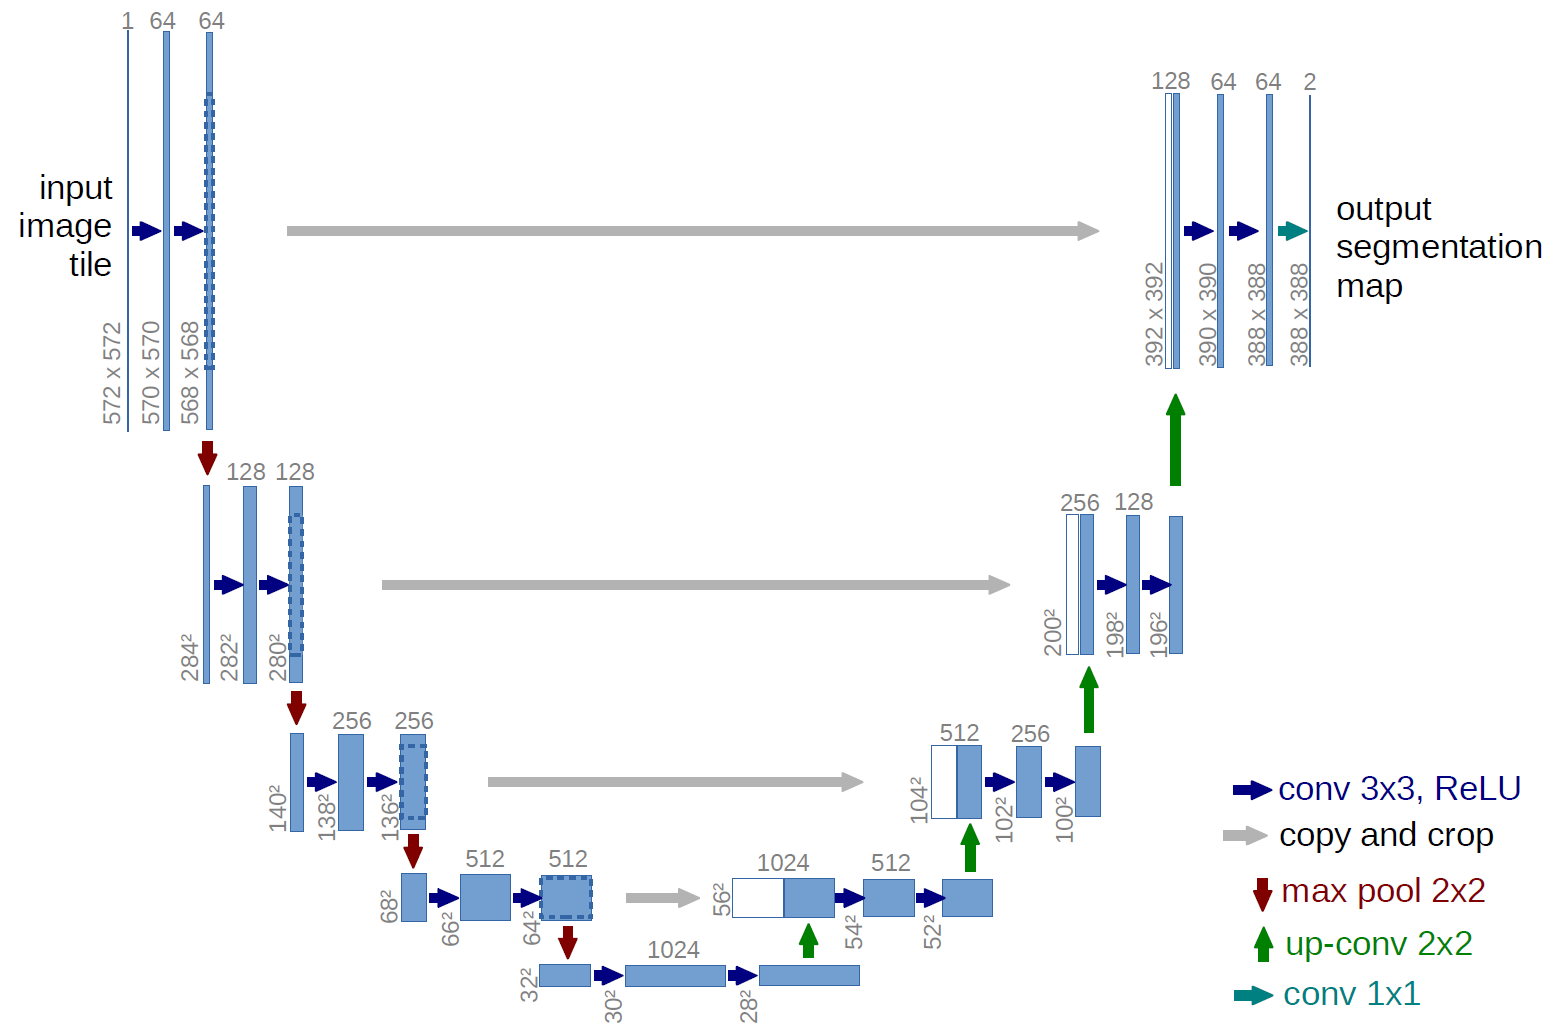
\includegraphics[width=0.8\textwidth]{unet-architecture.png}
	\end{figure}

\end{frame}


% Slide 3 ──────────────────────────────────────────────────────────────────────
\begin{frame}[t]

	\frametitle{Improved U-Net}

	Small improvements from previous $\rightarrow$ to reduce $n^{\circ}$ of
	parameters and improve performance:

	\vspace{4ex}

	\begin{itemize}
		 \setlength{\itemsep}{4ex}
		\item \bft{Separable Convolutions}: \gray{depthwise $+$ pointwise
			convolutions} 
		\item \bft{Batch Normalization}: \gray{to improve training and
			generalization}
		\item \bft{Larger Kernel Size}: \gray{$7 \times 7$ kernels instead of $3
			\times 3$}
		\item \bft{Inverse Bottleneck}: \gray{expands $+$ compresses channels}
		\item \bft{Additive Skip Connections}: \gray{instead of concatenated ones}
	\end{itemize}

\end{frame}


% Slide 4 ──────────────────────────────────────────────────────────────────────
\begin{frame}[t]

	\frametitle{Attention U-Net}

	% TODO: Also here replace figures with tikZ pictures highlighting important
	% elements covered in the speech

	\begin{figure}
		\centering
		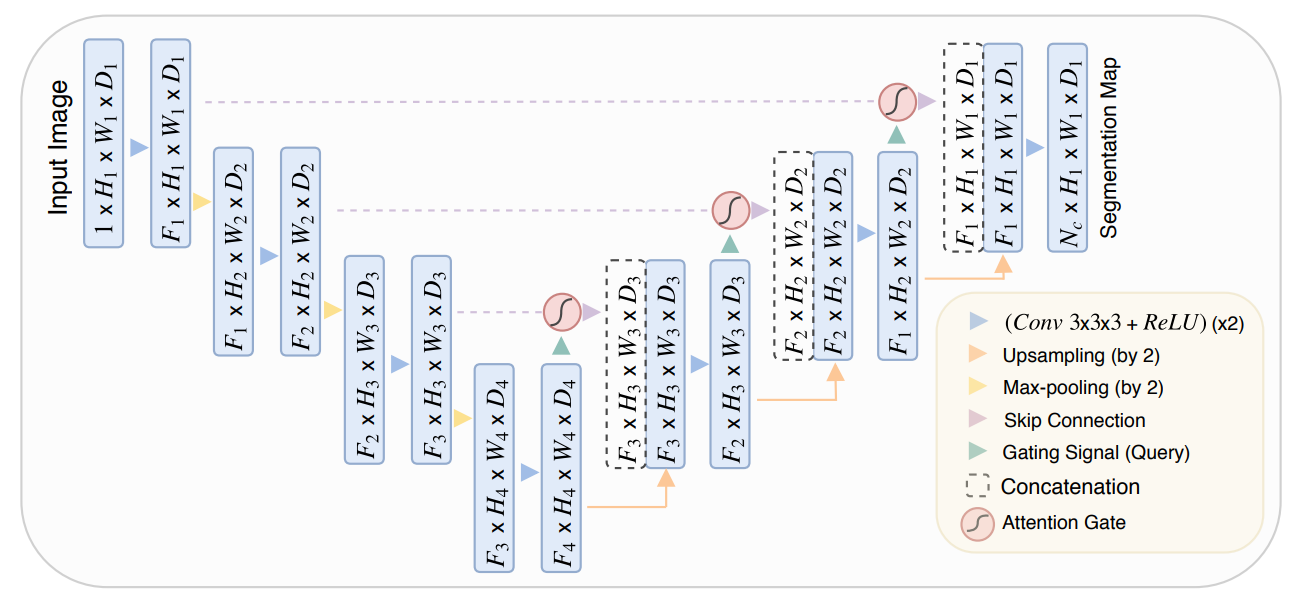
\includegraphics[width=0.8\textwidth]{attention-unet-architecture.png}
		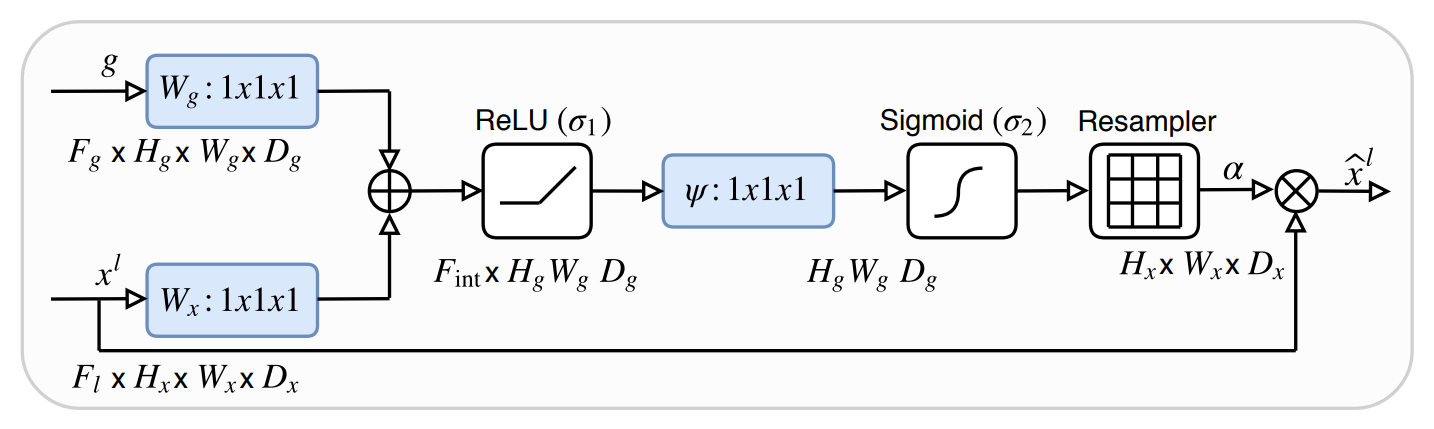
\includegraphics[width=0.8\textwidth]{attention-gate.png}
	\end{figure}

\end{frame}


% Slide 5 ──────────────────────────────────────────────────────────────────────
\begin{frame}[t]

	\frametitle{Training Details}

	U-Net Models training parameters:

	\begin{itemize}
		\setlength{\itemsep}{2ex}
		\item \bft{epochs}: $20$
		\item \bft{Optimizer}: Adam \gray{(with weight decay ($1 \times 10^{-2}$))}
		\item \bft{Scheduler}: Exponential Decay \gray{($\gamma = 0.9$)}
		\item \bft{Loss Function}: BCE with Logits Loss % TODO: formula HERE...
		\item \bft{learning rate}: $2 \times 10^{-3}$
		\item \bft{batch size}: $32$ \gray{(both training and validation)}
		\item \bft{image size}: $240 \times 240$
		\item \bft{first encoder filters}: $32$
	\end{itemize}

	% Just a test:
	% \begin{minipage}{0.23\textwidth}
	% 	\begin{cbox}
	% 		\begin{center}
	% 			% \bft{\huge{20}}\\
	% 			{\fontsize{20}{20}\selectfont{$20$}}\\
	% 			epochs
	% 		\end{center}
	% 	\end{cbox}
	% \end{minipage}
	% \begin{minipage}{0.28\textwidth}
	% 	\begin{cbox}
	% 		\begin{center}
	% 			learn~rate\\
	% 			{\fontsize{15}{30}\selectfont{$2 \cdot 10^{-3}$}}
	% 		\end{center}
	% 	\end{cbox}
	% \end{minipage}

\end{frame}


% Slide 6 ──────────────────────────────────────────────────────────────────────
\begin{frame}[t]

	\frametitle{Performance Assessment}

	\begin{equation*}
		\begin{array}{c c c c c}
			\text{Dice} = \frac{2 \times |X \cap Y|}{|X| + |Y|} & 
			\quad\quad &
			\text{Precision} = \frac{TP}{TP + FP} & 
			\quad\quad &
			\text{Recall} = \frac{TP}{TP + FN} \\[1em]
			\substack{
				\text{\gray{\itt{Dice Coefficient}}} \\[0.5em]
				\text{\azure{\itt{``overlap'' metric}}}
			} & &
			\substack{
				\text{\gray{\itt{Precision}}} \\[0.5em]
				\text{\azure{\itt{prediction quality}}}
			} & &
			\substack{
				\text{\gray{\itt{Recall}}} \\[0.5em]
				\text{\azure{\itt{prediction quantity}}}
			}
		\end{array}
	\end{equation*}

	% TODO: Plot of these 3 indexes as they change through epochs for the three
	% models (U-Net, Improved U-Net, Attention U-Net)
	% Recall to plot both for the singe channels and the average of all channels:
	% so maybe do 4 plots in total and do comparison in each of them

	% NOTE: Extra material: all the indexes plots of the other metrics

\end{frame}


% Slide 7 ──────────────────────────────────────────────────────────────────────
\begin{frame}[t]

	\frametitle{Visualizing Attention Maps}
	
	\begin{figure}
		\centering
		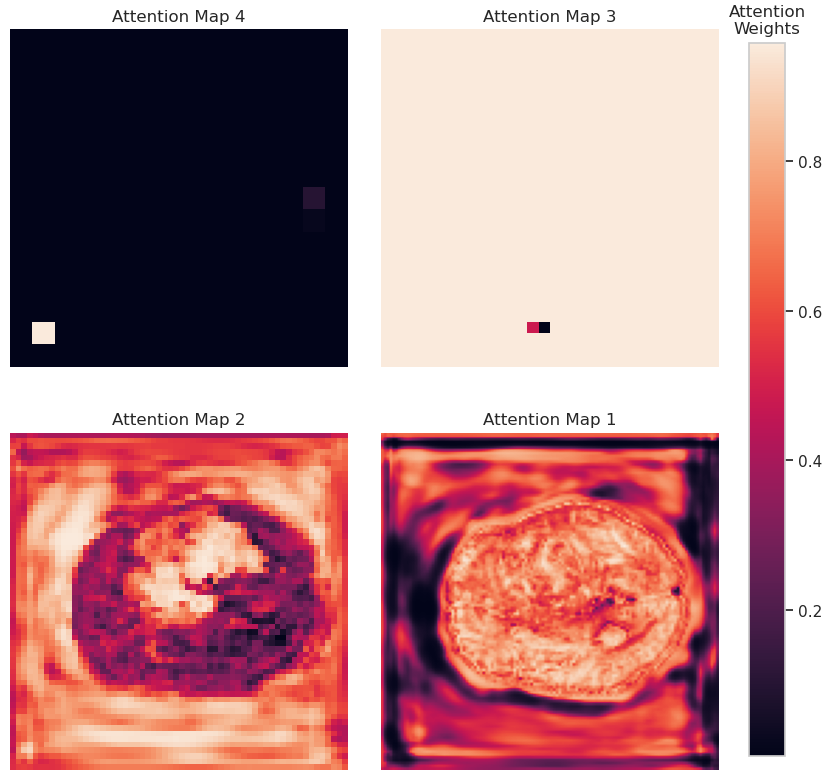
\includegraphics[width=0.7\textwidth]{attention-maps.png}
	\end{figure}

	% TODO: Probably better place these maps on a 1x4 grid for spacing

\end{frame}

\end{document}

